\documentclass[compress,color=usenames]{beamer}

\newcommand{\mytitlenbr}{1}
\newcommand{\mytitle}{Image Archive}

%\documentclass[compress,color=usenames,handout]{beamer}

%\usepackage{pgfpages}
%\pgfpagelayout{4 on 2}[a4paper,border shrink=5mm]

\usepackage{graphicx}
\usepackage{amsfonts,amssymb}
\usepackage{latexsym}
\usepackage{mdwtab}
\usepackage{xspace}
\usepackage{tikz}
\usetikzlibrary{shapes,snakes}
\usetikzlibrary{petri}

\DefineNamedColor{named}{Periwinkle}{cmyk}{0.57,0.55,0,0}
\DefineNamedColor{named}{Plum}{cmyk}{0.50,1,0,0}
\DefineNamedColor{named}{Red}{cmyk}{0,1,1,0}

\newcommand{\mH}[1]{\textcolor{Plum}{#1}}
\newcommand{\mT}[1]{\textcolor{Periwinkle}{#1}}

\newcommand{\tup}[1]{\langle #1 \rangle}

\newcommand{\dd}{{:}}
\newcommand{\I}{\mathcal{I}}
\newcommand{\csetsc}[2]{\{#1 $\mid$ #2\}}
\newcommand{\cset}[1]{\{#1\}}

\newcommand{\CON}{\textsf{CON}\xspace}
\newcommand{\ROL}{\textsf{ROL}\xspace}
\newcommand{\IND}{\textsf{IND}\xspace}
\newcommand{\PROP}{\textsf{PROP}\xspace}
\newcommand{\lang}{\mathcal{L}\xspace}


\newcommand{\mytt}[1]{\textsf{\scriptsize{#1}}}
\newcommand{\mytts}[1]{\textsf{\scriptsize{#1}}}

%\usefonttheme{serif}

\mode<presentation>
 {
 \usetheme{lined}
 }

\setbeamertemplate{navigation symbols}{}


\newcommand{\F}{\mathop{\mathsf{F}\vphantom{a}}\nolimits}
\newcommand{\G}{\mathop{\mathsf{G}\vphantom{a}}\nolimits}
\newcommand{\X}{\mathop{\mathsf{X}\vphantom{a}}\nolimits}

\newcommand{\Blue}[1]{\textcolor{blue}{#1}}
\newcommand{\Red}[1]{\textcolor{red}{#1}}
\newcommand{\Green}[1]{\textcolor{PineGreen}{#1}}


\title[GLN y Aplicaciones]{\Huge Generaci\'on de Lenguaje Natural y Aplicaciones}
%\mH{Lecture \#\mytitlenbr:} \mytitle}

\author[Areces \& Benotti]{
 Carlos Areces y Luciana Benotti\\[1ex]
\normalsize \url{{carlos.areces, luciana.benotti}@gmail.com}}

\institute[INRIA / UNC]{
INRIA Nancy Grand Est, Nancy, France\\
Universidad Nacional de C\'ordoba, C\'ordoba, Argentina}

\date{ELiC 2010 - Buenos Aires - Argentina}

\begin{document}


\beamerdefaultoverlayspecification{}


\begin{frame}[plain]
 \titlepage
\end{frame}

\begin{frame}
\frametitle{Lo que Vemos Hoy}

\begin{itemize}
\item Las Tareas B\'asicas de GLN
\item Tree Adjoining Grammars (TAGS)
\item TAGs for Natural Language Processing
\end{itemize}

\end{frame}

\begin{frame}
\frametitle{Lo que Veremos Hoy}

\begin{itemize}
\item \mH{Las Tareas B\'asicas de GLN}
\begin{tabular}{|l}
 Document Planning\\
 Microplanning\\
 Surface Realization\\
\end{tabular}

\item Tree Adjoining Grammars (TAGS)
\item TAGs for Natural Language Processing
\end{itemize}

\end{frame}

\begin{frame}
\frametitle{Las Tareas B\'asicas en un sistema de GLN}

\begin{center}
\begin{tabular}{|l|c|}  \hline
Content Determination & \mH{Document} \\
Document Structuring &  \mH{planning}\\ \hline
Aggregation &  \mH{Micro-}\\
Lexicalisation & \mH{planning}\\
Referring Expression Generation & \\ \hline
Linguistic Realisation & \mH{Surface}\\
Structure Realisation & \mH{realization}\\ \hline
\end{tabular}
\end{center}

\end{frame}


\begin{frame}
\frametitle{Y si nos Salteamos Microplanning?}

\begin{itemize}
\item Podr\'iamos saltearnos completamente la etapa de microplanning
\item Producimos una sentencia por cada mensaje del plan de documento
\begin{itemize}
\item Para cada tipo de mensaje en un nodo del plan decidimos, individualmente, como ser\'a realizado
\end{itemize}
\end{itemize}
 
\end{frame}

\begin{frame}
\frametitle{Ejemplo de un Document Plan}

\begin{center}
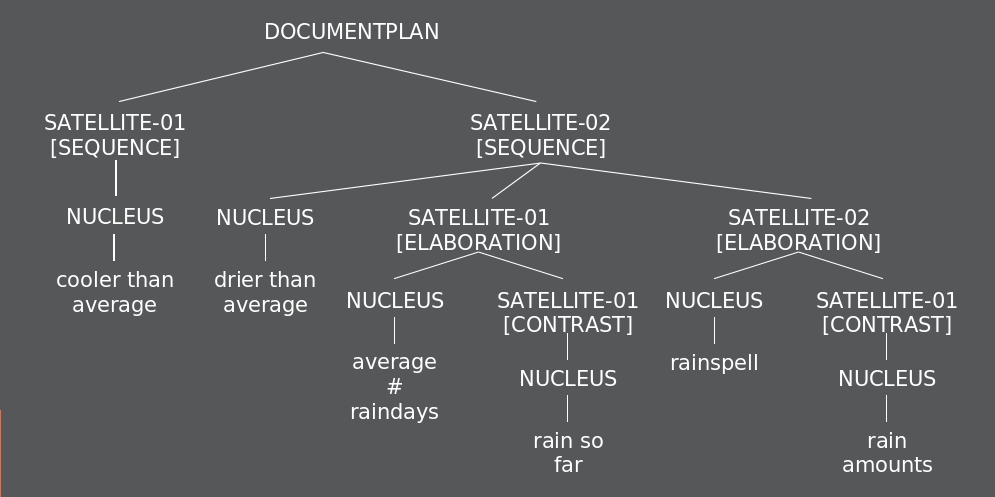
\includegraphics[scale=.4]{pics/pic10.jpg}
\end{center}
 
\end{frame}

\begin{frame}
\frametitle{Un Realizador Simple}

\begin{itemize}
\item { {Para el mensaje MonthlyTemperatureMsg:}}\\
{ {TempString = case (TEMP - AVERAGETEMP)}}
\ \ \ \begin{tabular}{ll}
 (2.0 -- 2.9): &`very much warmer than average.'\\
 (1.0 -- 1.9): &`much warmer than average.'\\
 (0.1 -- 0.9): &`slightly warmer than average.'\\
 (-0.1 -- -0.9): &`slightly cooler than average.'\\
 (-1.0 -- -1.9): &`much cooler than average.'\\
 (-2.0 -- -2.9): &`very much cooler than average.'
\end{tabular}

\item { {Sentencia = `The month was' + TempString}}
\end{itemize}
 
\end{frame}

\begin{frame}
\frametitle{Un Mensaje por Sentencia}

\begin{itemize}
\item { \mH{El resultado ser\'ia:}}

\ \ \ \  The month was cooler than average.\\
\ \ \ \  The month was drier than average.\\
\ \ \ \  There were the average number of rain days.\\
\ \ \ \  The total rain for the year so far is well below average.\\ 
\ \ \ \  There was rain on every day for 8 days from 11th to 18th.\\
\ \ \ \  Rainfall amounts were mostly small.\pause

\item { \mH{El texto target:}}
\begin{quote}
The month was cooler and drier than average, with the average number of rain days, but the total rain for the year so far is well below average. 
Although there was rain on every day for 8 days from 11th to 18th, rainfall amounts were mostly small.
\end{quote}
\end{itemize}
 
\end{frame}

%\begin{frame}
%\frametitle{El Problema de Usar Templates}

%Demos una mirada al corpus target. En nuestro caso de estudio, por ejemplo:

%\begin{itemize}
%\item MonthlyTemp y MonthlyRainfall no siempre aparecen en la misma sentencia
%\item Cuando aparecen en la misma sentencia, no siempre aparecen en el mismo orden
%\item Cada mensaje puede realizarse en formas diferentes: e.g., `very warm' vs. `warmer than average'
%\item Informaci\'on adicional puede o no incorporarse en la misma sentencia. 
%\end{itemize}
% 
%\end{frame}

\begin{frame}
\frametitle{Microplanning}

\label{f196}
\begin{itemize}
\item { \mH{Objetivo: }}
\begin{itemize}
\item Convertir el document plan en una secuencia de sentencias o especificaci\'on de frases.
\end{itemize}
\item { \mH{Tareas:}}
\begin{itemize}
\item Agregaci\'on de p\'arrafos y sentencias
\item Lexicalizaci\'on
\item Referencia 
\end{itemize}
\end{itemize}
 
\end{frame}

\begin{frame}
\frametitle{La Arquitectura}

\begin{center}
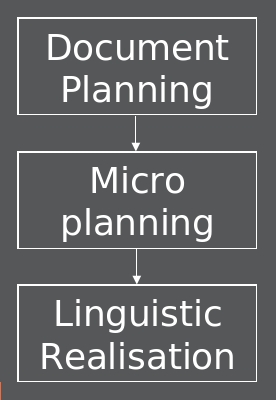
\includegraphics[scale=.4]{pics/pic11.jpg}
\end{center}
 
\end{frame}

\begin{frame}
\frametitle{Interacciones en Microplanning}

\begin{center}
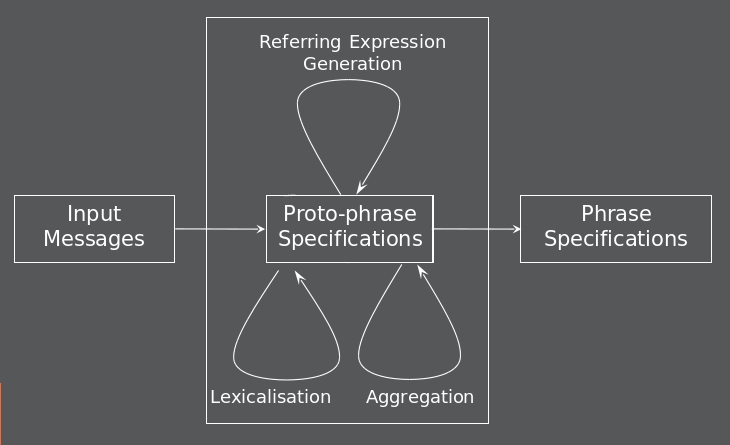
\includegraphics[scale=.4]{pics/pic12.jpg}
\end{center}
 
\end{frame}

\begin{frame}
\frametitle{Microplanning en un Pipeline}

\begin{center}
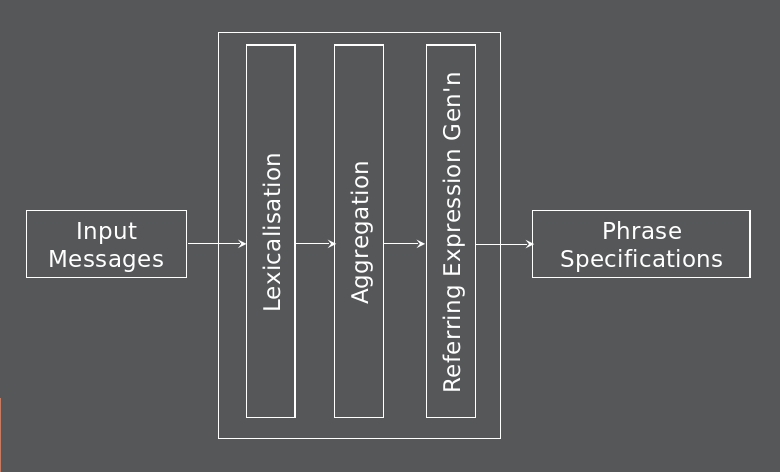
\includegraphics[scale=.4]{pics/pic13.jpg}
\end{center}
 
\end{frame}

\begin{frame}
\frametitle{Agregaci\'on}

\begin{itemize}
\item { \mH{Podemos combinar (agrupar) texto de acuerdo a}}
\begin{itemize}
\item { {el contenido de informaci\'on}}
\item { {posibilidades de realizaci\'on}}
\end{itemize}
\item { \mH{Algunas Posibilidades:}}
\begin{itemize}
\item { {Conjunci\'on}}
\item { {Elipsis}}
\item { {Embedding}}
\item { {Introducci\'on mediante Conjuntos}}
\end{itemize}
\end{itemize}
 
\end{frame}


\begin{frame}
\frametitle{Ejemplos}

\begin{itemize}
  \item { {Sin Agregaci\'on:}}
  \begin{itemize}
    \item Heavy rain fell on the 27th.\\
          Heavy rain fell on the 28th.
  \end{itemize}
\item { {Agregaci\'on via conjunci\'on simple:}}
\begin{itemize}
\item Heavy rain fell on the 27th and heavy rain fell on the 28th.
\end{itemize}
\item { {Agregaci\'on via elipsis: }}
\begin{itemize}
\item Heavy rain fell on the 27th and [] on the 28th.
\end{itemize}
\item { {Agregaci\'on via introducci\'on de conjuntos: }}
\begin{itemize}
\item Heavy rain fell on [the 27th and 28th].
\end{itemize}
\end{itemize}
 \end{frame}

\begin{frame}
\frametitle{Ejemplos: Embedding}

\label{f208}
\begin{itemize}
\item { {Sin agregaci\'on:}}
\begin{itemize}
\item March had a rainfall of 120mm.\\ 
It was the wettest month.
\end{itemize}
\item { {Con agregaci\'on:}}
\begin{itemize}
\item March, which was the wettest month, had a rainfall of 120mm.
\end{itemize}
\end{itemize}
 
\end{frame}

\begin{frame}
\frametitle{Heur\'isticas de Elecci\'on}

 Usualmente, hay muchas formas en que un conjunto de mensajes pueden agregarse: c\'omo elegimos? 

\label{f210}
\begin{itemize}
\item reglas convencionales y de estilo 
\item respetar propiedades estructurales 
\begin{itemize}
\item Por ejemplo, agregar solamente mensajes que son hermanos en el \'arbol del plan de documento
\end{itemize}
\item tomando en cuenta objetivos pragm\'aticos
\end{itemize}
 
\end{frame}

\begin{frame}
\frametitle{Objetivos Pragm\'aticos: STOP}

\label{f212}
\begin{itemize}
\item Hacer el texto m\'as amigable:
\begin{quote}
 It's clear from your answers that you don't feel too happy about being a smoker and it's excellent that you are going to try to stop.
\end{quote}
\item Hacer el texto m\'as simple (para personas con dificultades de lectura):
\begin{quote}
 It's clear from your answers that you don't feel too happy about being a smoker. It's excellent that you are going to try to stop.
\end{quote}
\end{itemize}
 
\end{frame}

\begin{frame}
\frametitle{Agregaci\'on en WeatherReporter}

\label{f214}
\begin{itemize}
\item Teniendo en cuenta las relaciones ret\'oricas:
\begin{itemize}
\item Si dos mensajes est\'an en la relaci\'on SEQUENCE, pueden ser agrupados al mismo nivel.
\item Si un mensaje es una ELABORATION de otro, puede ser agrupado al mismo nivel, o embebido como 
una clausula o frase menor. 
\item Si un mensaje es un CONTRAST de otro,  puede ser agrupado al mismo nivel, o embebido como 
una clausula o frase menor. 
\end{itemize}
\end{itemize}
 \end{frame}

\begin{frame}
\frametitle{Ejemplo de Regla de Agregaci\'on}

\begin{center}
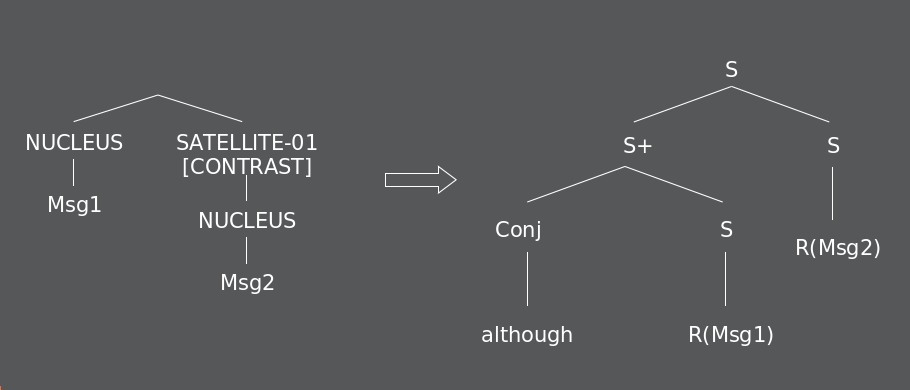
\includegraphics[scale=.4]{pics/pic14.jpg}
\end{center}
 
\end{frame}

\begin{frame}
\frametitle{Lexicalizaci\'on}

\begin{itemize}
\item Es el proceso de elecci\'on de palabras para comunicar la informaci\'on de un mensaje
\item { \mH{M\'etodos:}}
\begin{itemize}
\item templates
\item \'arboles de decisi\'on
\item algoritmos de reescritura de grafos
\end{itemize}
\end{itemize}
\end{frame}


\begin{frame}
\frametitle{Elecci\'on L\'exica}

Si m\'ultiples lexicalizaciones son posibles, considerar:

\begin{itemize}

\item el conocimiento del usuario y sus preferencias
\item consistencia con usos anteriores
\begin{itemize}
\item aunque en algunos casos, puede ser posible variar lexemas
\end{itemize}
\item interacci\'on con otros aspectos de microplanning
\item objetivos pragm\'aticos
\begin{itemize}
\item It is encouraging that you have many reasons to stop.\\ \hfill       \mH{(significado mas preciso)}
\item It's good that you have a lot of reasons to stop.\\ \hfill \mH{(m\'as f\'acil de leer)}
\end{itemize}
\end{itemize}

\end{frame}

\begin{frame}
\frametitle{WeatherReporter: Variaciones al describir MonthlyRainfallMsg}

\begin{itemize}
\item Variaciones en la \mH{categor\'ia sint\'actica}:

\ \ \  {{S:                [rainfall was very poor]}}\\
\ \ \  {{NP:        [a much worse than average rainfall]}}\\
\ \ \  {{AP:        [much drier than average]}}\\

\item {{Variaciones \mH{sem\'anticas}:}}

\ \ \ Valores absolutos:\\        
\ \ \ \ \ \                [very dry]\\
\ \ \ \ \ \                 [a very poor rainfall]\\

\ \ \ Valores comparativos:        \\
\ \ \ \ \ \ [a much worse than average rainfall]\\
\ \ \ \ \ \ [much drier than average] 
\end{itemize}
\end{frame}

\begin{frame}
\frametitle{WeatherReporter: Agregaci\'on y Lexicalizaci\'on}

Muchos resultados diferentes son posibles

\begin{quote}
{{The month was cooler and drier than average.
There were the average number of rain days, but the total rain for the year so far is well below average. There was rain on every day for 8 days from 11th to 18th, but rainfall amounts were mostly small.}}
\end{quote}

\begin{quote}
{{The month was cooler and drier than average.
Although the total rain for the year so far is well below average, there were the average number of rain days.  There was a small mount of rain on every day for 8 days from 11th to 18th.}}
\end{quote}

\end{frame}

\begin{frame}
\frametitle{Generaci\'on de Expresiones Referenciales}

Como identificamos objetos y entidades espec\'ificas del dominio?

\begin{itemize}
\item {{Dos temas que se discuten cl\'asicamente:}}
\begin{itemize}
\item \mH{Primera referencia} a un objeto
\item \mH{Referencias subsequentes} a un objeto previamente introducido (y `notorio')
\end{itemize}
\end{itemize}
\end{frame}

\begin{frame}
\frametitle{Referencia Inicial}

Introduciendo un objeto en el discurso

\begin{itemize}
\item {{usar un nombre completo}}
\begin{itemize}
\item Jeremy
\end{itemize}
\item relacionar con un objeto que ya fue introducido (y es notorio)
\begin{itemize}
\item Jane's goldfish
\end{itemize}
\item especificar ubicaci\'on f\'isica
\begin{itemize}
\item the goldfish in the bowl on the table
\end{itemize}
\end{itemize}

Un tema todav\'ia no resuelto, y en investigaci\'on.
\end{frame}

\begin{frame}
\frametitle{Referencias Subsequentes}

Algunas posibilidades

\begin{itemize}
\item {{Pronombres}}
\begin{itemize}
\item \underbar{It} swims in circles.
\end{itemize}
\item Frases nominales definidas (definite NPs)
\begin{itemize}
\item \underbar{The goldfish} swims in circles.
\end{itemize}
\item Nombres propios (quizas abreviados)
\begin{itemize}
\item \underbar{Jeremy} swims in circles.
\end{itemize}
\end{itemize}
\end{frame}

\begin{frame}
\frametitle{Eligiendo el Modo de Referencia}

Algunas sugerencias en la literatura:
\begin{itemize}
\item usar un pronombre si este refiere a una entidad mencionada en la frase anterior, siempre y cuando no hay otra entidad en la frase anterior que pueda ser referica con el mismo pronombre
\item si no, usar un nombre, si este existe
\item si no, generar un definite NP
\end{itemize}

Tambi\'en es importante seguir las convenciones del g\'enero -- por ejemplo, se usan m\'as pronombres en art\'iculos period\'isticos que en manuales t\'ecnicos 
\end{frame}

\begin{frame}
\frametitle{Ejemplo}

\begin{quote}
 {{I am taking the Caledonian Express tomorrow.  \underbar{It} is a much better train than the Grampian Express.  \underbar{The Caledonian} has a real restaurant car, while \underbar{the Grampian} just has a snack bar.   \underbar{The restaurant car} serves wonderful fish, while \underbar{the snack bar} serves microwaved mush.}}
\end{quote}
\end{frame}

\begin{frame}
\frametitle{Generaci\'on de Expresiones Referenciales en WeatherReporter}

\begin{itemize}
\item {{Referencias a meses:}}
\begin{itemize}
\item June 1999
\item June
\item the month
\item next June
\end{itemize}
\item Relativamente simple, puede harcodearse durante la etapa de document planning
\end{itemize}
\end{frame}

\begin{frame}
\frametitle{Temas de Investigaci\'on}

\begin{itemize}
\item C\'omo guiar las elecciones durante microplanning?
\item C\'omo hacer agregaci\'on de alto nivel, i.e., como formar parrafos a partir de sentencias?
\item C\'omo guiar las elecciones de lexicalizaci\'on, en particular, como lexicalizar cuando 
conceptos del dominio no pueden traducirse directamente y en forma f\'acil en palabras? 
\item Cu\'al es la mejor manera de referirnos a un objeto (en particular en una primera referencia)?
\end{itemize}
\end{frame}

\begin{frame}
\frametitle{La Arquitectura}

\begin{center}
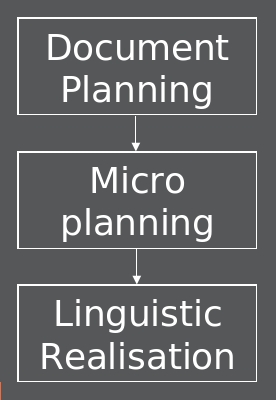
\includegraphics[scale=.4]{pics/pic11.jpg}
\end{center}
 
\end{frame}


\begin{frame}
\frametitle{Realizaci\'on}

\label{f23}
\begin{itemize}
\item {\mH{Objetivo: }}
\begin{itemize}
\item Convertir las especificaciones de texto en texto en lenguaje natural
\end{itemize}
\item {\mH{Motivo: }}
\begin{itemize}
\item intentar separar lo m\'as posible las particularidades de un lenguaje dado, del resto del sistema de GLN
\end{itemize}
\end{itemize}
\end{frame}

\begin{frame}
\frametitle{Tareas de Realizaci\'on}

\begin{itemize}
\item {\mH{Realizaci\'on de Estructura:}}
  \begin{itemize}
  \item Elegir el markup necesario para transmitir la estructura del documento
  \end{itemize}
\item {\mH{Realizaci\'on Ling\"u\'istica:}}
\begin{itemize}
\item Insertar palabras funcionales (functional words). E.g., art\'iculos, preposiciones, etc.
\item Elegir la inflexi\'on correcta de las palabras de contenido (content words). E.g., sustantivos, adjetivos, etc.
\item Ordenar las palabras dentro de una frase
\item Aplicar reglas ortogr\'aficas y morfol\'ogicas (inflexion de palabras, reglas de puntuaci\'on, etc.)

\end{itemize}
\end{itemize}
\end{frame}

\begin{frame}
\frametitle{Realizaci\'on de Estructura}

\begin{itemize}
\item Agregar \mH{markup} al documento:
\item Ejemplo: formas de marcar el fin de p\'arrafo
\begin{center}
\begin{tabular}{ll}
 HTML  &                       \mbox{$<$}P\mbox{$>$}\\
 LaTeX  &                       (blank line)\\
 RTF     &                   \mbox{$\backslash$}par\\
 SABLE (speech) &       \mbox{$<$}BREAK\mbox{$>$}\\
\end{tabular}
\end{center}
\item Depende del formato en que se representar\'a el documento
\item Usualmente puede resolverse con reglas simples de mapeo
\end{itemize}
\end{frame}

\begin{frame}
\frametitle{Realizaci\'on Ling\"u\'istica}

Diferentes t\'ecnicas:
\begin{itemize}
\item Especificaci\'on de \mH{gram\'aticas bidireccionales}
\item Especificaci\'on de \mH{gram\'aticas espec\'ificas para generaci\'on} 
\item Mecanismos basados en \mH{templates}
\end{itemize}
\end{frame}

\begin{frame}
\frametitle{Especificaci\'on de Gram\'aticas Bidireccionales}

\label{f31}
\begin{itemize}
\item \mH{Idea Principal}: Utilizaci\'on de una misma gram\'atica para realizaci\'on y parsing
\item Puede ser expresada como un conjunto de mapeos declarativos entre estructuras sint\'acticas y sem\'anticas
\item Lo que diferir\'a (generaci\'on vs.\ interpretaci\'on) ser\'an los algoritmos que utilicen la gram\'atica 
\item Elegantes en teor\'ia
\item Hoy en d\'a, son utilizadas en algunos sistemas de traducci\'on autom\'atica, pero casi nunca en sistemas de GLN aplicada.
\begin{itemize}
\item Dificultad de construir gram\'aticas bidireccionales de gran tama\~no
\item Dificultad de generar frases espec\'ificas con estas gram\'aticas
\end{itemize}
\end{itemize}
\end{frame}

\begin{frame}
\frametitle{Gram\'aticas Especialmente Definidas para Generaci\'on}

\label{f35}
\begin{itemize}
\item La gram\'atica provee un \mH{\'arbol de decisi\'on} para la realizaci\'on
\item Las elecciones se hacen en base a la especificaci\'on en el plan del documento
\item Estas gram\'aticas se pueden utilizar \mH{s\'olo para generaci\'on}
\item Existe software y estandares para construir estas gram\'aticas
\end{itemize}
\end{frame}

\begin{frame}
\frametitle{Observaci\'on}

\begin{itemize}
\item Los dos enfoques anteriores apuntan a generar texto de amplia 
cobertura ling\"u\'istica y de car\'acter sofisticado.
\item La mayor\'ia de las aplicaciones no require este nivel de sofisticaci\'on: 
en muchos casos los objetivos de generaci\'on se pueden obtener via templates o `canned text' 
\item Lo que si puede suceder es que ciertas partes del problema de generaci\'on requiera 
m\'as sofisticaci\'on que otras.
\item En muchos casos la soluci\'on  es combinar canned text, templates y `realizaci\'on en serio' 
\end{itemize}
 
\end{frame}

\begin{frame}
\frametitle{Temas de Investigaci\'on}

\label{f67}
\begin{itemize}
\item C\'omo combinamos distintas t\'ecnicas y formalismos ling\"u\'isticos?
\item Cu\'ales son los costos y beneficions de usar templates en vez de `realizaci\'on en serio'?
\item En qu\'e casos hay interacci\'on entre realizaci\'on de estructura y realizaci\'on ling\"u\'istica?
\end{itemize}
 
\end{frame}

%\begin{frame}
%\frametitle{Lo que Veremos Hoy}

%\begin{itemize}
%\item  Introducci\'on a GLN 
%\item  Un Caso de Estudio
%\item  Las Tareas b\'asicas de GLN
%\item  GLN en Ambientes Multimedia y Multimodales
%\end{itemize}
%\end{frame}

%\begin{frame}
%\frametitle{
%Document Types}

%\label{f71}
%\begin{itemize}
%\item {{Simple ASCII (eg email messages)}}
%\begin{itemize}
%\item relatively straightforward: just words and punctuation symbols
%\end{itemize}
%\item {{Printed documents (eg newspapers, technical documents)}}
%\begin{itemize}
%\item need to consider typography, graphics
%\end{itemize}
%\item {{Online documents (eg Web pages)}}
%\begin{itemize}
%\item need to consider hypertext links
%\end{itemize}
%\item {{Speech (eg radio broadcasts, information by telephone)}}
%\begin{itemize}
%\item need to consider prosody
%\end{itemize}
%\item {{Visual presentation (eg TV broadcasts, MS Agent)}}
%\begin{itemize}
%\item need to consider animation, facial expressions
%\end{itemize}
%\end{itemize}
 
%\end{frame}

%\begin{frame}
%\frametitle{
%Typography}

%\label{f73}
%\begin{itemize}
%\item {{Character attributes (italics, boldface, colour, font)}}
%\begin{itemize}
%\item can be used to indicate emphasis or other aspects of use:  typographic distinctions carry meaning
%\end{itemize}
%\item {{Layout (itemised lists, section and chapter headings)}}
%\begin{itemize}
%\item allows indication of structure, can enable information access
%\end{itemize}
%\item {{Special constructs provide sophisticated resources}}
%\begin{itemize}
%\item boxed text, margin notes, ...
%\end{itemize}
%\end{itemize}
% 
%\end{frame}

%\begin{frame}
%\frametitle{
%Typographically-flat Text}

%\label{f75}
%\begin{itemize}
%\item {{When time is limited, travel by limousine, unless cost is also limited, in which case go by train.  When only cost is limited a bicycle should be used for journeys of less than 10 kilometers, and a bus for longer journeys.  Taxis are recommended when there are no constraints on time or cost, unless the distance to be travelled exceeds 10 kilometers.  For journeys longer than 10  kilometers, when time and cost are not important, journeys should be made by hire car.}}
%\end{itemize}
% 
%\end{frame}

%\begin{frame}
%\frametitle{
%Structured Text}

%\label{f77}
%\begin{itemize}
%\item {{\textit{When only time is limited}:}}
%\begin{itemize}
%\item travel by Limousine
%\end{itemize}
%\item {{\textit{When only cost is limited}:}}
%\begin{itemize}
%\item travel by Bus if journey more than10 kilometers
%\item travel by Bicycle if journey less than10 kilometers
%\end{itemize}
%\item {{\textit{When both time and cost are limited}:}}
%\begin{itemize}
%\item travel by Train
%\end{itemize}
%\item {{\textit{When time and cost are not limited}:}}
%\begin{itemize}
%\item travel by Hire Car if journey more than10 kilometers
%\item travel by Taxi if journey less than10 kilometers
%\end{itemize}
%\end{itemize}
% 
%\end{frame}

%\begin{frame}
%\frametitle{
%Tabular Presentation}

%\label{f79}
% 
%\end{frame}

%\begin{frame}
%\frametitle{
%Diagrammatic Presentation}

%\label{f81}
% 
%\end{frame}

%\begin{frame}
%\frametitle{
%Text and Graphics}

%\label{f83}
%\begin{itemize}
%\item {{Which is better?  Depends on:}}
%\begin{itemize}
%\item type of information communicated
%\item expertise of user
%\item delivery medium
%\end{itemize}
%\item {{Best approach: use both!}}
%\end{itemize}
% 
%\end{frame}

%\begin{frame}
%\frametitle{
%An Example from WIP}

%\label{f85}
% 
%\end{frame}

%\begin{frame}
%\frametitle{
%Similarities between
%Text and Graphics}

%\label{f87}
%\begin{itemize}
%\item {{Both contain sublanguages}}
%\item {{Both permit conversational implicature}}
%\item {{Structure is important in both}}
%\item {{Both express discourse relations}}
%\item {{Do we need a media-independent theory of communication?}}
%\end{itemize}
% 
%\end{frame}

%\begin{frame}
%\frametitle{
%Hypertext}

%\label{f89}
%\begin{itemize}
%\item {{Generate Web pages!}}
%\begin{itemize}
%\item Dynamic hypertext
%\end{itemize}
%\item {{Models of hypertext}}
%\begin{itemize}
%\item browsing
%\item question-space
%\item dialogue
%\end{itemize}
%\item {{Model-dependent issues}}
%\begin{itemize}
%\item click on a link twice: same result both times?
%\item discourse models for hypertext
%\end{itemize}
%\end{itemize}
% 
%\end{frame}

%\begin{frame}
%\frametitle{Example:  Peba}

%\label{f91}
% 
%\end{frame}

%\begin{frame}
%\frametitle{
%Speech Output}

%\label{f93}
%\begin{itemize}
%\item {{The GLN Perspective: enhances output possibilities}}
%\begin{itemize}
%\item communicate via spoken channels (eg, telephone)
%\item add information (eg emotion, importance)
%\end{itemize}
%\item {{The speech synthesis perspective: intonation carries information}}
%\begin{itemize}
%\item Need information about syntactic structure, information status, homographs
%\item Currently obtained by text analysis
%\item Could by obtained from an GLN system automatically:  the idea of concept-to-speech
%\end{itemize}
%\end{itemize}
% 
%\end{frame}

%\begin{frame}
%\frametitle{
%Examples}

%\label{f95}
%\begin{itemize}
%\item {{\textit{John took a bow}}}
%\begin{itemize}
%\item Difficult to determine which sense of \textit{bow} is meant, and therefore how to pronounce it, from text analysis
%\item But an GLN system knows this
%\end{itemize}
%\item {{\textit{John washed the dog}}}
%\begin{itemize}
%\item Should stress that part of the information that is new
%\item An GLN system will know what this is
%\end{itemize}
%\end{itemize}
% 
%\end{frame}


%\begin{frame}
%\frametitle{Lo que Veremos Hoy}

%\begin{itemize}
%\item  Introducci\'on a GLN 
%\item  Un Caso de Estudio
%\item  Las Tareas b\'asicas de GLN
%\item  GLN en Ambientes Multimedia y Multimodales
%\end{itemize}
%\end{frame}


%\begin{frame}
%\frametitle{
%GLN en la Actualidad}

%\label{f99}
%\begin{itemize}
%\item {{Many GLN applications being investigated }}
%\item {{Few actually fielded}}
%\begin{itemize}
%\item but at least there are some: in 1989 there were none
%\end{itemize}
%\item {{We are beginning to see reusable software, and specialist software houses}}
%\item {{More emphasis on mixing simple and complex techniques}}
%\item {{More emphasis on evaluation}}
%\item {{We believe the future is bright}}
%\end{itemize}
% 
%\end{frame}

%\begin{frame}
%\frametitle{
%Resources: SIGGEN}

%\label{f101}
%\begin{itemize}
%\item {{SIGGEN (ACL Special Interest Group for Generation)}}
%\item {{Web site at  
%http://www.dynamicmultimedia.com.au/siggen}}
%\begin{itemize}
%\item resources: software, papers, bibliographies
%\item conference and workshop announcements
%\item job announcements
%\item discussions
%\item GLN people and places
%\end{itemize}
%\end{itemize}
% 
%\end{frame}

\begin{frame}
\frametitle{Lo que Vemos Hoy}

\begin{columns}
\column{1.2\textwidth}
\begin{itemize}
\item Las Tareas B\'asicas de GLN
\item \mH{Tree Adjoining Grammars (TAG)}
\item TAGs for Natural Language Processing
\end{itemize}
\end{columns}
\end{frame}

\begin{frame}
\frametitle{Lo que Vemos Hoy}

\begin{columns}
\column{1.2\textwidth}
\begin{itemize}
\item Las Tareas B\'asicas de GLN
\item \mH{Tree Adjoining Grammars (TAG)}
\begin{tabular}{|l}
Capacidad Generativa D\'ebil vs. Fuerte\\
Introduciendo TAG\\
Propiedades de TAG, Complejidad\\
Lexicalizaci\'on de Gram\'aticas
\end{tabular}

\item TAGs y Surface Realization
\end{itemize}
\end{columns}
\end{frame}

\begin{frame}
\frametitle{Gram\'aticas Formales}

\begin{itemize}
\item Podemos usar gram\'aticas formales para \mH{generar} lenguages.  
\item Por ejemplo la gram\'atica 
\begin{center}
\begin{tabular}{rcl}
$S$ & $\to$ & $aSb \mid ab$
\end{tabular}
\end{center}
genera $a^nb^n$ para $n\ge 1$
\item Podemos usar este tipo de gram\'aticas \mH{para generar lenguaje natural}?
\end{itemize}
\end{frame}

\begin{frame}
\frametitle{John loves Mary}

\begin{center}
\begin{tabular}{rcl}
  S & $\rightarrow$ & NP VP \\

 VP & $\rightarrow$ & V NP $\mid$ VP ADV  \\

 NP & $\rightarrow$ & John $\mid$ Mary  \\

  V & $\rightarrow$ & loves \\

ADV & $\rightarrow$ & passionately 
\end{tabular}
\end{center}


$L(G)$ = \{John loves Mary, John loves Mary passionately,\ldots\} 

\end{frame}


\begin{frame}
\frametitle{Gram\'aticas Formales}

\begin{itemize}
\item Recordemos de todas formas que la tarea de GLN es 
\begin{itemize}
\item Transformar \mH{informaci\'on no ling\"u\'istica}
\item en \mH{texto comprensible en lenguaje natural}
\end{itemize}
\item Podemos usar este tipo de gram\'atica para generar a partir de informaci\'on no 
ling\"u\'istica?
\item Que gram\'atica tenemos que usar?
\end{itemize}
\end{frame}

\begin{frame}
\frametitle{La Jerarqu\'ia de Chomsky}

Una gram\'atica $G$ es una tupla $(N, T, R, S)$ donde 
\begin{itemize}
\item $N$ es un conjunto de s\'imbolos (\mH{No Terminales})
\item $T$ es el conjunto de s\'imbolos disjunto de $N$ (\mH{Terminales})
\item $R$ es una relacion en $(N\cup T)^* \times (N\cup T)^*$
\item $S$ es un s\'imbolo de $N$. \pause 
\end{itemize}

Sea $G = (N, T, R, S)$ una gram\'atica donde  $\alpha$, $\beta$, $\gamma$ $\in$ $(N \cup T)^*$

\begin{itemize}
\item unrestricted o type-0 grammars: $\alpha$ $\rightarrow$ $\beta$, tal que $\alpha \not = \epsilon$

\item context-sensitive grammars: $\alpha$A$\beta$ $\rightarrow$ $\alpha$$\gamma$$\beta$, tal que $\gamma \not = \epsilon$

\item context-free grammars: A $\rightarrow$ $\gamma$

\item regular grammars: A $\rightarrow$ a B or A $\rightarrow$ a

\end{itemize}

\end{frame}

\begin{frame}
\frametitle{Qu\'e Gram\'atica Tenemos que Usar}

\begin{itemize}
\item Olvidemonos por un momento del \mH{problema de generaci\'on}.
\item Supongamos que queremos escribir una gram\'atica que \mH{contenga} un lenguaje natural como el Ingles o 
el Castellano
\item Es decir una gram\'atica $G$ tal que $L(G)$ sea un \mH{subconjunto interesante} de un lenguaje natural
\item Que \mH{tipo} de gram\'atica tiene que ser $G$? E.g., puede ser una gram\'atica regular? 
\end{itemize}
\end{frame}


\begin{frame}
\frametitle{Capacidad Generativa D\'ebil vs.\ Fuerte}

\begin{itemize}
\item Que queremos generar? $L(G)$ o $T(G)$

\item La \mH{capacidad generativa d\'ebil $L(G)$} de una gram\'atica es el 
conjunto de strings (o lenguaje) que la gram\'atica genera/reconoce, e.g.\ $0^n1^n$ para $n \geq 0$

\item La \mH{capacidad generativa fuerte $T(G)$} de una gram\'atica es el 
conjunto de derivaciones (usualmente un conjunto de \'arboles) de una gram\'atica
\end{itemize}
\end{frame}

\begin{frame}
\frametitle{Capacidad Generativa D\'ebil vs. Fuerte}

\begin{center}
\begin{tabular}{rcl}
  S & $\rightarrow$ & NP VP \\

 VP & $\rightarrow$ & V NP $\mid$ VP ADV  \\

 NP & $\rightarrow$ & John $\mid$ Mary $\mid$ David $\mid$ peanuts \\

  V & $\rightarrow$ &  loves $\mid$ likes\\

ADV & $\rightarrow$ & passionately 
\end{tabular}
\end{center}


L(G) = \{David likes peanuts, David likes peanuts passionately,\ldots\}

\end{frame}

\begin{frame}
\frametitle{Arbol Derivado / Arbol de Parsing}

\begin{center}
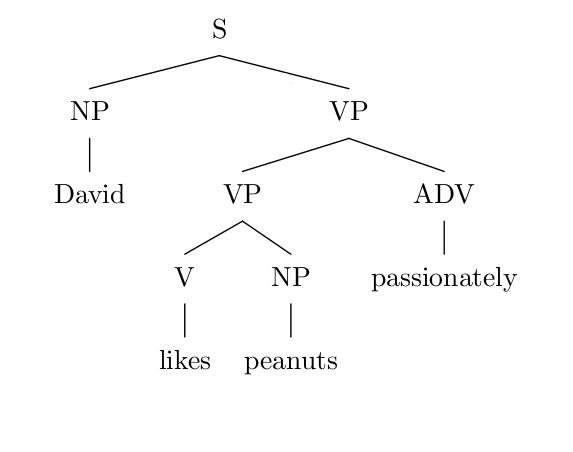
\includegraphics[scale=.4]{pics/pic2-1.jpg}
\end{center}
\end{frame}

\begin{frame}
\frametitle{No Confundir con: Arbol de Derivaci\'on}

\begin{center}
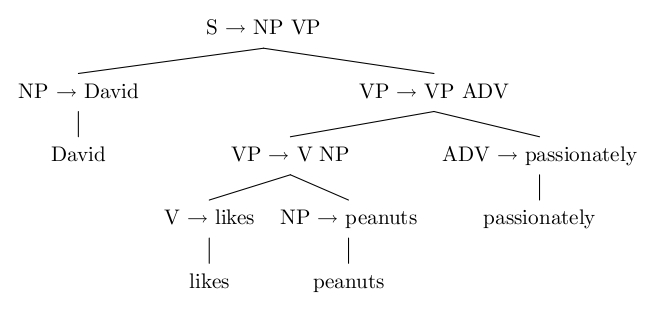
\includegraphics[scale=.4]{pics/pic2-2.jpg}
\end{center}
\end{frame}

\begin{frame}
\frametitle{Mismo $L(G)$, Distinto $T(G)$} 

Dos gram\'aticas pueden tener el mismo $L(G)$ pero distingo $T(G)$ 

\begin{center}
\begin{tabular}{rcl}
$S$ & $\rightarrow$ & $AB$\\
$A$ & $\rightarrow$ & $aA$ $\mid$ $a$\\
$B$ & $\rightarrow$ & $Bb$ $\mid$ $b$
\end{tabular}
\end{center}

$L(G) = a^+b^+$ \hspace*{1cm} $T(G) = $
\begin{picture}(100,30)
\put(0,-70){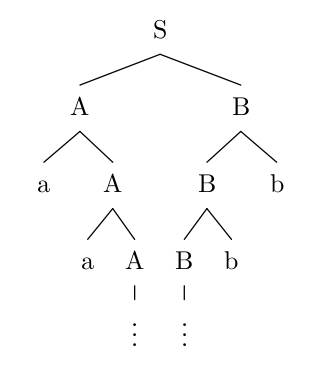
\includegraphics[scale=.3]{pics/pic2-3.jpg}}
\end{picture}

\end{frame}

\begin{frame}
\frametitle{Lenguaje Natural y Complejidad Descriptiva}


\begin{itemize}

\item La pregunta que nos estamos haciendo entonces es: existe algun tipo 
de lenguaje formal que \mH{describa} (al menos ciertos aspectos de un fragmento de) un
lenguaje natural?

\item Por ejemplo, supongamos que podemos abstraer algun fen\'omeno ling\"u\'istico
de tal forma que lo podemos representar como el lenguaje
$$\{ww^R \mid \mbox{ donde } w \in \{a, b\}^*, w^R \mbox{ es el reverso de } w\}$$ 

\item Podemos representar este lenguaje con una gram\'atica regular? O necesitamos 
subir en la jerarqu\'ia?

\end{itemize}
\end{frame}

\begin{frame}
\frametitle{M\'as All\'a de Libre de Contexto}

\begin{itemize}
\item Actualmente, se considera que ciertos aspectos de muchos lenguajes naturales
\mH{no pueden ser modelados} mediante gram\'aticas libres de contexto

\item Si consideramos la capacidad generativa fuerte (i.e., $T(G)$) mostrar este 
resultado es relativamente simple.
\begin{itemize}
\item Los lenguajes libres de contexto no pueden generar lenguajes con `dependencias cruzadas.' 
E.g., $a^nb^mc^nd^m$
\item Es relativamente f\'acil dar ejemplos de $T(G)$ correspondientes a fen\'omenos ling\"u\'isticos
con dependencias cruzadas.
\end{itemize}

\end{itemize}

\end{frame}

\begin{frame}
\frametitle{M\'as All\'a de Libre de Contexto}

\begin{itemize}
\item Pero un resultado sobre capacidad generativa fuerte necesariamente 
est\'a asociado a \mH{una determinada teor\'ia ling\"u\'istica} (e.g., analisar\'a 
sentencias de una forma determinada, usando ciertas categor\'ias gramaticales)

\item No sabemos \mH{qu\'e teor\'ia ling\"u\'istica es la correcta}!

\item Lo \'unico que conocemos son las sentencias que producimos, el resto est\'a 
solo en nuestras cabezas. 

\item Por eso, un resultado m\'as fuerte (y m\'as interesante) ser\'ia poder 
demostrar que cierto lenguaje natural no es libre de contexto a nivel de capacidad generativa d\'ebil.
\end{itemize}
\end{frame}

\begin{frame}
\frametitle{M\'as All\'a de Libre de Contexto en $L(G)$}

\begin{itemize}

\item Pero demostrar esto es dif\'icil

\item Consideremos 
$L_1 = \{a^nb^n\}$ es libre de contexto mientras que $L_2 = \{a^*b^*\}$ es
regular y $L_1 \subset L_2$.

\item Es decir, podriamos `hacer trampa' y elegir algun subset del lenguaje natural 
particularmente dif\'icil para demostrar nuestro resultado, mientras que el \mH{lenguaje completo} tiene menor complejidad. 

\end{itemize}
\end{frame}

%\begin{frame}
%\frametitle{Strong vs. Weak Generative Capacity}

%\begin{itemize}
%\item Also, if we consider the size of a grammar then also the answer is easier
%to obtain (*joyable, *richment). The CFG is more elegant and smaller
%than the equivalent regular grammar:

%\begin{center}
%\begin{tabular}{rcl}
% V & $\rightarrow$ & X\\

% A & $\rightarrow$ & X -able $\mid$ X -ment\\

% X & $\rightarrow$ & en- NA\\

%NA & $\rightarrow$ & joy $\mid$ rich\\
%\end{tabular}
%\end{center}

%\item This is an engineering argument. However, it is related to the problem of
%describing the human learning process. Certain aspects of language are
%learned all at once not individually for each case.
%e.g., learning enjoyment automatically if enrichment was learnt
%\end{itemize}

%\end{frame}

\begin{frame}
\frametitle{El Lenguaje Humano no es un Lenguaje Libre de Contexto}

\begin{itemize}

\item Existen en la literatura diferentes argumentos e intentos de 
demostraci\'ion de que la capacidad generativa d\'ebil del lenguaje humano
est\'a mas alla de las gram\'aticas libres de contexto.

\item (Pullum, 1982) es un compedio de muchos de estos argumentos y de sus 
problemas.

\item (Shieber, 1985) y (Huybregts, 1984) proveyeron finalmente un 
argumento fuerte utilizando ejemplos de Alem\'an-Suizo.
\end{itemize}

\end{frame}



\begin{frame}
\frametitle{Ejemplo: M\'as alla de Lenguajes Regulares}

\begin{itemize}
\item Consideremos  `center embedding' en Ingl\'es 


\begin{center}
the shares that the broker recommended were bought\\ $\Rightarrow$\\ $N_1N_2V_2V_1$


the moment when the shares that the broker recommended were bought
has passed\\ $\Rightarrow$\\ $N_1N_2N_3V_3V_2V_1$\pause
\end{center}

\item Podemos modelar este tipo de frases con una gram\'atica como 
$$S \rightarrow a S b$$ 

que produce dependencias anidadas como en $a_1a_2a_3b_3b_2b_1$\pause

\item Cu\'antas veces podemos anidar de esta forma? Por ejemplo, podemos 
construir una frase que suene natural y que incluya cuatro verbos? 
\end{itemize}
\end{frame}

\begin{frame}
\frametitle{Competencia vs.\ Performance}

\begin{itemize}
\item Que pasa si no podemos embeber m\'as de 3 o 4 sentencias? 

\item Si existe 
un limite finito (no importa que grande sea), entonce si podemos modelar 
este fragmento usando un lenguaje regular!

\item Usualmente vamos a querer diferenciar \mH{competencia} 
de \mH{performance}. I.e., lo que consideramos gramaticalmente correcto, de lo 
que realmente producimos (dadas, por ejemplo, nuestras limitaciones de memoria).

\item En el caso anterior dir\'iamos que la performance puede modelarse con 
un lenguaje regular, mientras que la competencia necesita un lenguaje libre de 
contexto.
\end{itemize}

\end{frame}

\begin{frame}
\frametitle{Ejemplo: Mas all\'a de Libre de Contexto}

\begin{itemize}
\item Varios lenguajes tienen dependencias cruzadas:
Holandes (Bresnan et al., 1982), Alem\'an-Suizo (Shieber, 1984), Tagalog
(Rambow and MacLachlan, 2002)\pause

\item Alem\'an-Suizo:
\begin{center}
\begin{tabular}{llllll}
... & mer & em Hans & es huss   & halfed & aastriiche \\
... & we  & Hans    & the house & helped & paint\\
    & \multicolumn{2}{c}{$N_1$} & 
      \multicolumn{1}{c}{$N_2$} &
      \multicolumn{1}{c}{$V_1$} & 
      \multicolumn{1}{c}{$V_2$}
\end{tabular}

we helped Hans paint the house
\end{center}

\end{itemize}

\end{frame}

\begin{frame}
\frametitle{Lo que Vemos Hoy}

\begin{columns}
\column{1.2\textwidth}
\begin{itemize}
\item Las Tareas B\'asicas de GLN
\item Tree Adjoining Grammars (TAG)
\begin{tabular}{|l}
Capacidad Generativa D\'ebil vs. Fuerte\\
\mH{Introduciendo TAG}\\
Propiedades de TAG, Complejidad\\
Lexicalizaci\'on de Gram\'aticas
\end{tabular}

\item TAGs y Surface Realization
\end{itemize}
\end{columns}
\end{frame}


\begin{frame}
\frametitle{Gram\'aticas de Arboles}

\begin{itemize}

\item En la discusion anterior usamos ambos $L(G)$ and $T(G)$ para discutir
distintos aspectos del lenguaje humano.

\item Como dijimos, \mH{sabemos} lo que $L(G)$ es y solo podemos \mH{teorizar}
hacerca de lo que $T(G)$ es. \pause

\item Pero una vez que fijamos una teor\'ia ling\"u\'istica, intuitivamente $T(G)$ 
es \mH{tan important o m\'as} que $L(G)$. 

\item De alguna forma, podemos decir que $L(G)$ es solo \mH{el resultado} de 
las caracter\'isticas de $T(G)$.  \pause

\item Resulta entonces raro que $T(G)$ sea solo algo `derivado' en la gram\'atica. 
Por que no tenemos gram\'aticas \mH{cuyo lenguaje sea $T(G)$}. 

\end{itemize}
\end{frame}

\begin{frame}
\frametitle{Gram\'atias de Arboles}

\begin{itemize}

\item En vez de construir \'arboles usando reglas de la gram\'atica, representamos
la regla \mH{directamente como un \'arbol}

\item Usaremos \mH{\'arboles elementales} como unidades b\'asicas que pueden utilizarse
para reescribir no terminales en otros \'arboles elementales.

\item La reescritura es equivalente a la expansion de un no-terminal en una 
gram\'atica libre de contexto.  

\end{itemize}

\end{frame}

\begin{frame}
\frametitle{Arboles Finitos Ordenadios Etiquetados}

\begin{itemize}
\item Un \'arbol finito ordenado etiquetado es una estructura $t = \tup{N_t, \triangleleft_t, \prec_t, L_t}$ 
donde\pause

\begin{itemize}
\item $N_t$ es un conjunto finito no vac\'io de \mH{nodos} \pause

\item $\triangleleft_t$ y $\prec_t$ son \mH{relaciones binarias} sobre $N_t$, respectivamente `dominio' (dominance) y `precedencia' (precedence) \pause

\item $\triangleleft^t$ define un \'arbol (i.e., un \'unico nodo ra\'iz y todo nodo excepto la ra\'iz tiene un \'unico predecesor) y $\prec_t$ define un orden total sobre los hijos de un nodo. \pause

\item $L_t$ es la \mH{funci\'on de etiquetado}, que asigna a cada nodo un conjunto de etiquetas.  
\end{itemize}
\end{itemize}
\end{frame}

\begin{frame}
\frametitle{Elementos de una TAG}

Una TAG es un conjunto finito de arboles finitos ordenados etiquetados 
con ciertas caracteristicas

\begin{columns}
\column{.65\textwidth}

\begin{itemize}
\item Tomemos dos conjuntos $V_N$ (no terminales) y $V_T$ (terminales), finitos no vac\'ios \pause

\begin{picture}(0,0)
\only<2>{
\put(175,-82){
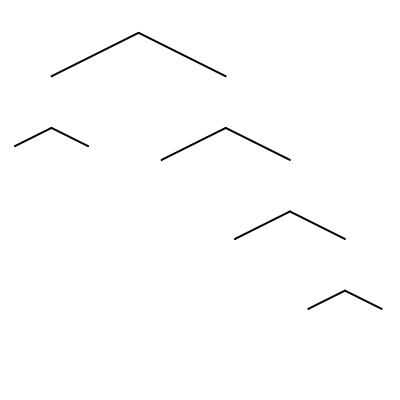
\includegraphics[scale=.5]{pics/pic2-9.jpg}
}}
\only<3>{
\put(175,-74){
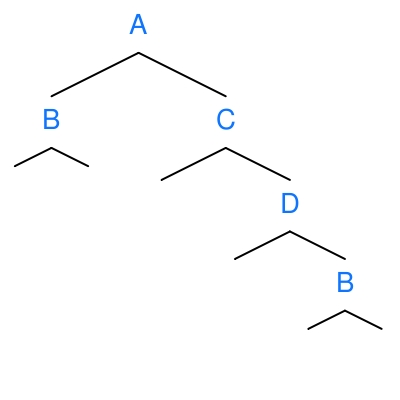
\includegraphics[scale=.5]{pics/pic2-10.jpg}
}}
\only<4>{
\put(172,-74){
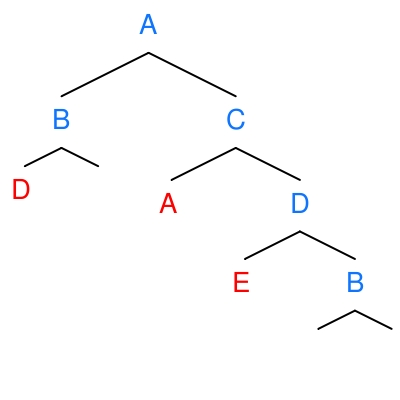
\includegraphics[scale=.5]{pics/pic2-11.jpg}
}}
\only<5>{
\put(172,-74){
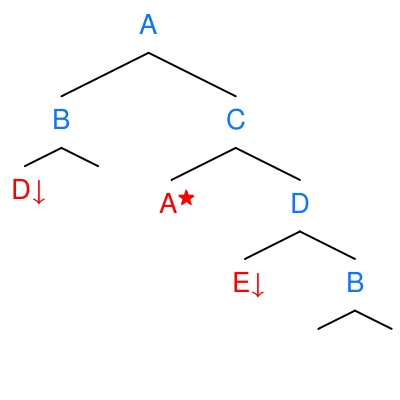
\includegraphics[scale=.5]{pics/pic2-12.jpg}
}}
\only<6>{
\put(172,-74){
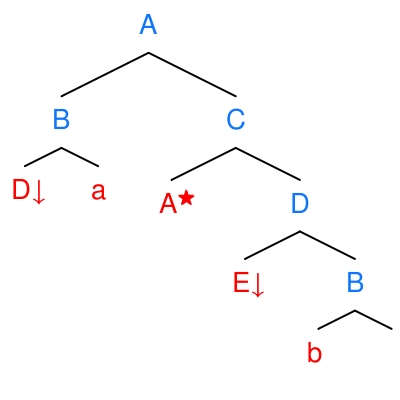
\includegraphics[scale=.5]{pics/pic2-13.jpg}
}}
\only<7>{
\put(172,-74){
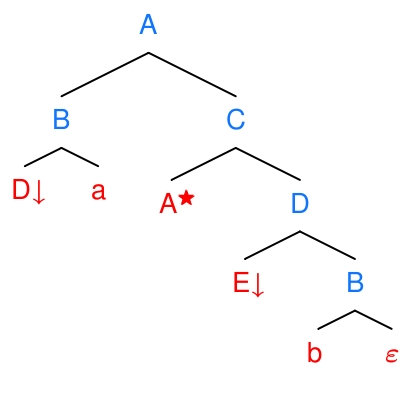
\includegraphics[scale=.5]{pics/pic2-14.jpg}
}}
\end{picture}

\vspace*{-.5cm}
\item $t = \tup{N_t, \triangleleft_t,\prec_t,L_t}$ \pause

\item $L_t$ :

\ \ \ NonLeaves$_t$ $\to$ \mH{$V_N$} \pause

\ \ \ Leaves$_t$$\to$\mH{$V_N$}$\pause\mH{\{\downarrow,\star\}}$\pause \mH{$\cup V_T$}\pause \mH{$\cup \{\epsilon\}$} 
\end{itemize}



\column{.5\textwidth}

\end{columns}
\end{frame}

\begin{frame}
\frametitle{Derivaciones en TAG}

\begin{itemize}
\item Podemos derivar nuevos arboles etiquetados mediante la aplicaci\'on de 
las operaciones de \mH{sustituci\'on} y \mH{adjunci\'on}.\pause

\item Usando \mH{\'arboles iniciales}

\begin{tabular}{l}
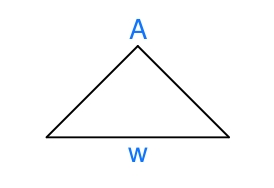
\includegraphics[scale=.5]{pics/pic2-15.jpg}
\end{tabular}
\begin{tabular}{l}
$A \in V_N$\\
$w \in (V_N \{\downarrow \} \cup V_T)^+$\pause
\end{tabular}

\item Y \mH{\'arboles auxiliares}

\begin{tabular}{l}
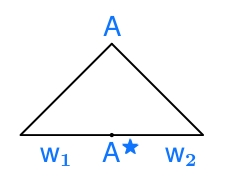
\includegraphics[scale=.5]{pics/pic2-16.jpg}
\end{tabular}
\begin{tabular}{l}
$A \in V_N$\\
$w_1,w_2 \in (V_N \{\downarrow \} \cup V_T)^+$
\end{tabular}

\end{itemize}
\end{frame}

\begin{frame}
\frametitle{Substituci\'on}

\begin{center}
\begin{tabular}{|c|c|} \hline
From & We obtain \\ \hline

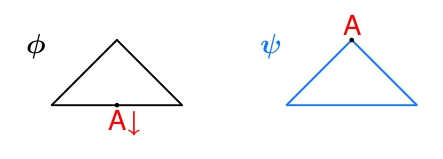
\includegraphics[scale=.4]{pics/pic2-17.jpg} & 

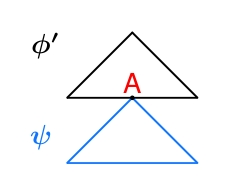
\includegraphics[scale=.4]{pics/pic2-18.jpg} \\ \hline

\multicolumn{2}{|c|}{by substituci\'on}  \\ \hline
\end{tabular}
\end{center}\pause


\mH{Ejemplo:}\begin{tabular}{l}
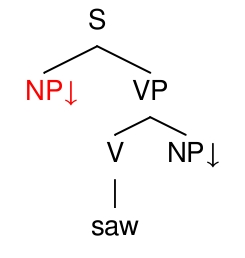
\includegraphics[scale=.4]{pics/pic2-19.jpg} \ \ \ \ \ \
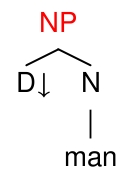
\includegraphics[scale=.4]{pics/pic2-20.jpg} \ \ \ \ \ \ 
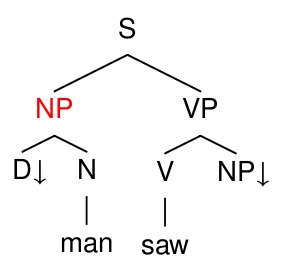
\includegraphics[scale=.4]{pics/pic2-21.jpg} 
\end{tabular}

\begin{picture}(0,0)
\put(120,40){+}
\put(190,40){$\Rightarrow$}
\end{picture}

\end{frame}

\begin{frame}
\frametitle{Adjunci\'on}


\begin{center}
\begin{tabular}{|c|c|} \hline
From & We obtain \\ \hline

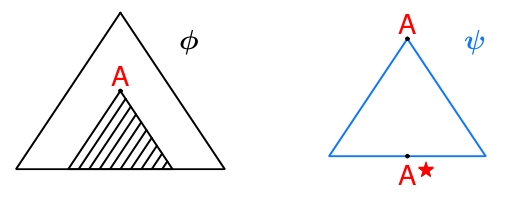
\includegraphics[scale=.4]{pics/pic2-22.jpg} & 

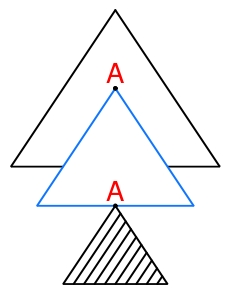
\includegraphics[scale=.35]{pics/pic2-23.jpg} \\ \hline

\multicolumn{2}{|c|}{by adjunci\'on}  \\ \hline
\end{tabular}
\end{center}\pause

\mH{Ejemplo:}\begin{tabular}{l}
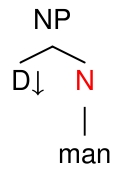
\includegraphics[scale=.45]{pics/pic2-24.jpg} \ \ \ \ \ \
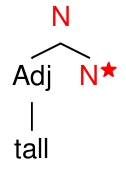
\includegraphics[scale=.45]{pics/pic2-25.jpg} \ \ \ \ \ \ 
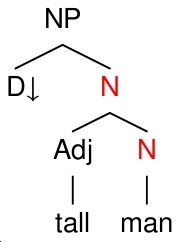
\includegraphics[scale=.45]{pics/pic2-26.jpg} 
\end{tabular}

\begin{picture}(0,0)
\put(90,40){+}
\put(155,40){$\Rightarrow$}
\end{picture}


\end{frame}


\begin{frame}
\frametitle{Tree Adjoining Grammar: Definici\'on Formal}

\begin{itemize}

\item Una Tree Adjoining Grammar es una tupla $G = (S , N, T, I, A)$ donde\pause

\begin{itemize}
\item $V_N$ es un conjunto de \mH{s\'imbolos no terminales}

\item $V_T$ es un conjunto de \mH{terminales} (disjunto de $N$)\pause

\item $I$ es un conjunto de \mH{\'arboles iniciales} 

\item $A$ es un conjunto de \mH{\'arboles auxiliares}\pause

\item $I \cup A$ es el conjunto de \mH{\'arboles elementales}\pause

\item $S$ (\mH{start}) es un \'arbol inicial $S \in I$

\end{itemize}

\end{itemize}
\end{frame}

\begin{frame}
\frametitle{Ejemplo}

\begin{center}
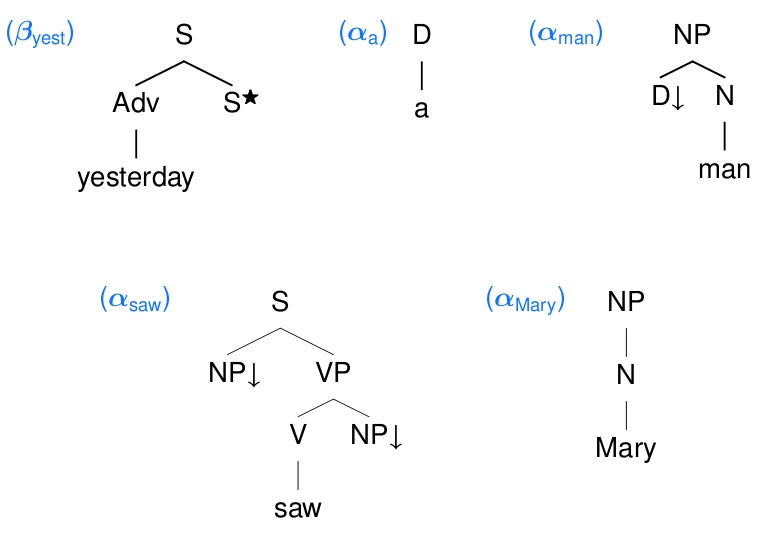
\includegraphics[scale=.45]{pics/pic2-27.jpg} 
\end{center}
\end{frame}

\begin{frame}
\frametitle{Lenguaje Generado por una TAG}

\begin{itemize}
\item El \mH{lenguaje generado} por una TAG:
\begin{itemize}
\item es el conjunto de \'arboles que pueden obtenerse \mH{a partir del \'arbol inicial}
\item utilizando las operaciones de \mH{sustituci\'on} y  \mH{adjunci\'on}
\item tales que sus hojas son \mH{todos s\'imbolos terminales}. 
\end{itemize} 

\item A partir del \mH{lenguaje de \'arboles} de una TAG podemos obtener un 
\mH{lenguaje de strings} considerando la `frontera' (?)  

\item \mH{Extensi\'ones habituales}: 
\begin{itemize}
\item Ciertos nodos no terminales pueden estar marcados como $na$ indicando 
que una operaci\'on de adjunci\'on no puede aplicarse en ese nodo
\item Ciertos nodos no terminales pueden estar marcados como permitiendo adjunciones 
s\'olo con cierto conjunto de \'arboles auxiliares.
\end{itemize}
\end{itemize}
\end{frame}

\begin{frame}
\frametitle{Lo que Vemos Hoy}

\begin{columns}
\column{1.2\textwidth}
\begin{itemize}
\item Las Tareas B\'asicas de GLN
\item Tree Adjoining Grammars (TAG)
\begin{tabular}{|l}
Capacidad Generativa D\'ebil vs. Fuerte\\
Introduciendo TAG\\
\mH{Propiedades de TAG, Complejidad}\\
Lexicalizaci\'on de Gram\'aticas
\end{tabular}

\item TAGs y Surface Realization
\end{itemize}
\end{columns}
\end{frame}


\begin{frame}
\frametitle{Tree Adjoining Grammars}

\begin{itemize}
\item Su poder expresivo est\'a entre las gram\'aticas libres de contexto y 
las sensibles al contexto

\item Pueden manejar todos los casos que mencionamos anteriormente de capacidad
generativa d\'ebil y fuerte de lenguajes naturales. 

\item Permite modelar f\'acilmente casos de dependencias cruzadas y anidadas.

\end{itemize}
\end{frame}

\begin{frame}
\frametitle{Dependencias Cruzadas en TAG: $a_2a_1b_2b_1$}

\begin{center}
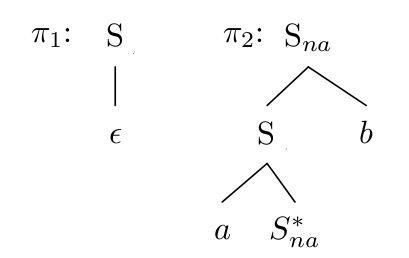
\includegraphics[scale=.4]{pics/pic2-4.jpg}
\end{center}

$$G : (T = \{a, b,\epsilon \}, N = \{S \}, I = \{\pi_1\}, A = \{\pi_2\}, S = \{\pi_1\})$$

\end{frame}

\begin{frame}
\frametitle{Dependencias Cruzadas en TAG}

\begin{center}
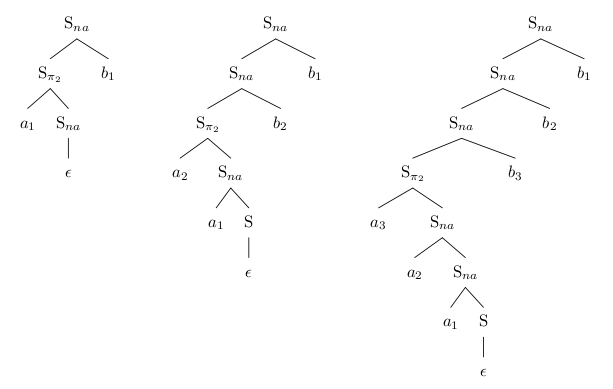
\includegraphics[scale=.4]{pics/pic2-5.jpg}
\end{center}


\end{frame}


\begin{frame}
\frametitle{Dependencias Anidadas en TAG: $c_1c_2d_2d_1$}


\begin{center}
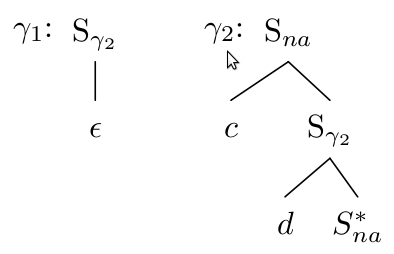
\includegraphics[scale=.4]{pics/pic2-6.jpg}
\end{center}
$$G : (T = \{c, d, \epsilon\}, N = \{S \}, I = \{\gamma_1\}, A = \{\gamma_2\}, S = \{\gamma_1\})$$\pause


\mH{Ejercicio} ver que podemos generar con una gram\'atica que contenga 
$\pi_1$, $\pi_2$, $\gamma_1$, y $\gamma_2$?

\end{frame}

\begin{frame}
\frametitle{Nos Ubicamos}

\begin{itemize}

\item context-sensitive grammars: 
\medskip
\centerline{$0^i$, $i$ no es primo y $i > 0$}\pause

\item indexed grammars: 
\medskip
\centerline{$0^n1^n2^n \ldots m^n$, para cualquier $m$ fijo y $n \geq 0$}\pause


\item tree-adjoining grammars (TAG): 
\medskip
\centerline{$0^n1^n2^n3^n$, para $n \geq 0$}\pause

\item context-free grammars: 
{$0^n1^n$ para $n \geq 0$}\pause


\item deterministic context-free grammars: 
\medskip
\begin{center}
$S \rightarrow \epsilon \mid Sc \mid S A \mid A$,\\
$A \rightarrow a S b \mid ab$\\ 
el lenguaje de par\'entesis balanceados \pause
\end{center}

\item regular grammars: 
{$(0\mid 1)^*00(0\mid 1)^*$}

\end{itemize}

\end{frame}

\begin{frame}
\frametitle{Nos Ubicamos}

\begin{center}
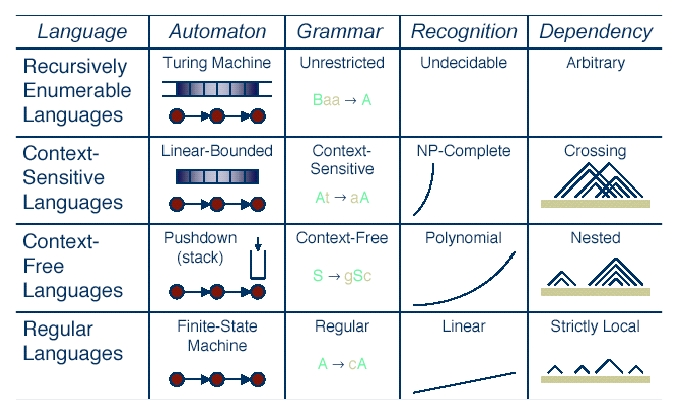
\includegraphics[scale=.4]{pics/pic2-7.jpg}
\end{center}


TAG esta entre CSL y CFG: puede ser reconocido en tiempo polinomial y puede
representar dependencias cruzadas.
\end{frame}

\begin{frame}
\frametitle{Complejidad}

\mH{Problema:} Dada una gram\'atica $G$ y un input $x$, determinar $x \in L(G)$

\begin{itemize}
\item unrestricted: indecidible\pause 

\item context-sensitive: NSPACE[n] -- linear non-deterministic space \pause


\item indexed grammars: NP-Complete \pause


\item tree-adjoining grammars (TAG): $O(n^6)$ \pause


\item context-free: $O(n^3)$ \pause

\item deterministic context-free: $O(n)$ \pause

\item regular grammars: $O(n)$

\end{itemize}

\end{frame}

\begin{frame}
\frametitle{Propiedades de TAG}

\begin{itemize}

\item Pertenencia est\'a en P (como dijimos es $O(n^6)$) \pause

\item TALs (los lenguajes de string obtenidos mediante TAGs) estan cerrados 
por union, concatenaci\'on, clausura de Kleene, h, h$^{-1}$, intersecci\'on
con RLs \pause

\item TALs no est\'an cerrados bajo intersecci\'on, intersecci\'on con CFLs 
ni complementaci\'on

\end{itemize}

\end{frame}

\begin{frame}
\frametitle{Formalismos Gramaticales Restringidos}

\begin{itemize}

\item Por que nos interesa definir el formalismo gramatical m\'as 
restringido que nos permita modelar lenguaje natural? \pause

\item Y si no nos importa el costo computacional?

\item Por ejemplo, un ling\"u\'ista podr\'ia usar el formalismo m\'as 
general posible para analysar un lengauje, sin preocuparse de `cuanto cuesta' 
computar ese modelo. 

\pause Si fuera necesario, podr\'iamos despues ver si podemos traducir 
(`implementar') ese modelo a un formalismo computacionalmente eficiente. 

\end{itemize}
\end{frame}

\begin{frame}
\frametitle{Formalismos Gramaticales Restringidos}

\begin{itemize}

\item En algunos casos, el formalismo gramatical nos puede ayudar proveyendo 
\mH{restricciones de que puede o no pasar}. 

\item Si el formalismo esta cercano a c\'omo producimos el lenguaje, el mismo 
formalismo nos da pistas de como modelar cierto fen\'omeno.

\item En otras palabras, un modelo err\'oneo deber\'ia ser mas d\'ificil de
escribir en un formalismo gramatical restringido, siempre y cuando ese formalismo 
este pr\'oximo a LA VERDAD. 

\item En otras, otras palabras, en un formalismo flexible es facil escribir 
tanto modelos correctos como incorrectos. 

\end{itemize}
\end{frame}

\begin{frame}
\frametitle{Lo que Vemos Hoy}

\begin{columns}
\column{1.2\textwidth}
\begin{itemize}
\item Las Tareas B\'asicas de GLN
\item Tree Adjoining Grammars (TAG)
\begin{tabular}{|l}
Capacidad Generativa D\'ebil vs. Fuerte\\
Introduciendo TAG\\
Propiedades de TAG, Complejidad\\
\mH{Lexicalizaci\'on de Gram\'aticas}
\end{tabular}

\item TAGs y Surface Realization
\end{itemize}
\end{columns}
\end{frame}

\begin{frame}
\frametitle{Gram\'aticas Lexicas}

\begin{itemize}
\item Decimos que una gramatica $G$ esta \mH{lexicalizada} si cada 
regla de $G$ contiene un terminal. \pause

\item Este tipo de gram\'aticas son especialmente \'utiles para parsing
\begin{itemize}
\item al observar un terminal en el string a parsear podemos directamente 
restringir el conjunto de reglas de la gram\'atica que pueden usarse para 
cubrirlo 
\end{itemize}

\item \mH{Pregunta}: Dada una gram\'atica arbitraria $G$, es posible encontrar
una gram\'atica $G'$ lexicalizada tal que $L(G) = L(G')$? \pause

\item Si $G$ es una CFG la respuesta es afirmativa: usar la Forma Normal de Griebach

\begin{quote}
Toda CFG puede ser reescrita de forma que sus reglas sean del tipo  $A \to a \alpha$ 
donde $a$ es un terminal.  
\end{quote} 

\end{itemize}
\end{frame}


\begin{frame}
\frametitle{Lexicalizaci\'on de TAGs}

\begin{itemize}

\item (Joshi and Schabes, 1997) muestran que TALs estas cerradas bajo lexicalizaci\'on:
\begin{quote}
toda TAL tiene una TAG lexicalizada que genera el mismo lenguaje. \pause
\end{quote}

\item La idea de lexicalizaci\'on es atractiva desde varias perspectivas
\begin{itemize}
\item sint\'axis
\item sem\'antica (en Ling\"u\'istica)
\item procesamiento y producc\'ion (en psicoling\"u\'istica)\pause
\end{itemize}

\item Intuitivamente, lo que estamos diciendo es que cada palabra codifica un entorno 
local de restricciones sint\'acticas y sem\'anticas. 

\item Muchos consideran esta intuici\'on acertada y una TAG parece particularmente 
apropiada para capturarla. 

\end{itemize}
\end{frame}

\begin{frame}
\frametitle{Ejemplo: TAG L\'exica}

\begin{center}
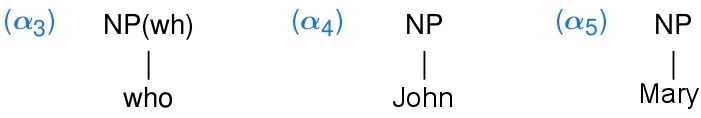
\includegraphics[scale=.35]{pics/pic2-30.jpg} \pause
\medskip

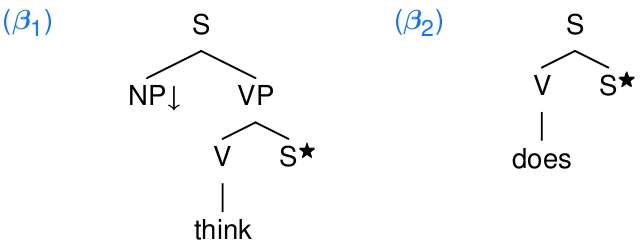
\includegraphics[scale=.35]{pics/pic2-29.jpg} \pause
\medskip

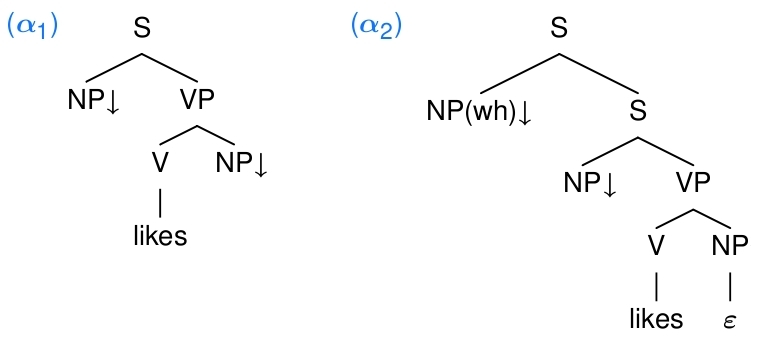
\includegraphics[scale=.35]{pics/pic2-28.jpg}

\end{center}
\end{frame}

%\begin{frame}
%\frametitle{Lexicalized Tree Adjoining Grammars}

%\begin{center}
%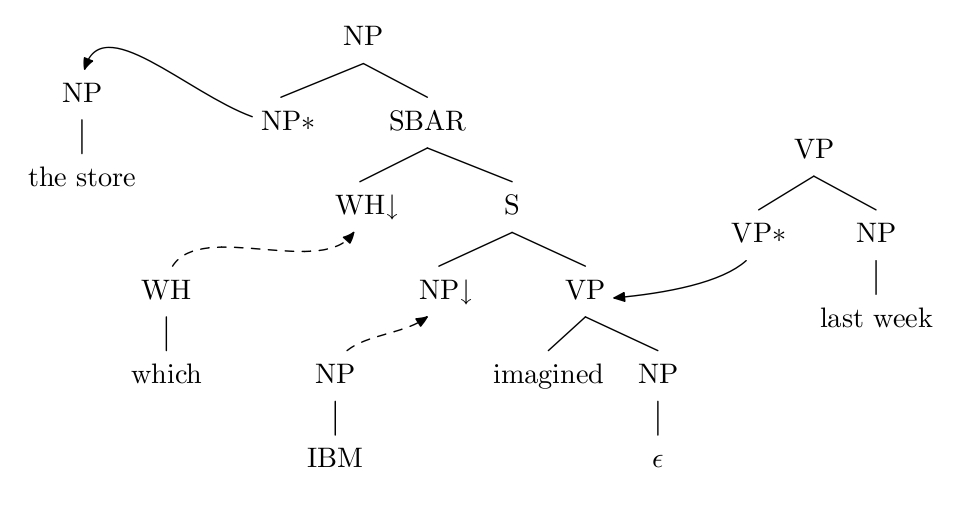
\includegraphics[scale=.4]{pics/pic2-8.jpg}
%\end{center}

%\end{frame}

\begin{frame}
\frametitle{Lo que Vemos Hoy}

\begin{itemize}
\item Las Tareas B\'asicas de GLN
\item Tree Adjoining Grammars (TAG)
\item \mH{TAGs y Surface Realization}
\end{itemize}
\end{frame}

\begin{frame}
\frametitle{Lo que Vemos Hoy}

\begin{itemize}
\item Las Tareas B\'asicas de GLN
\item Tree Adjoining Grammars (TAG)
\item TAGs y Surface Realization
\begin{tabular}{|l}
Inteface sint\'actica / sem\'antica\\
Unificaci\'on\\
Algoritmo de Realizaci\'on
\end{tabular}
\end{itemize}
\end{frame}

\begin{frame}
\frametitle{El Algoritmo de Realizaci\'on}

\begin{center}
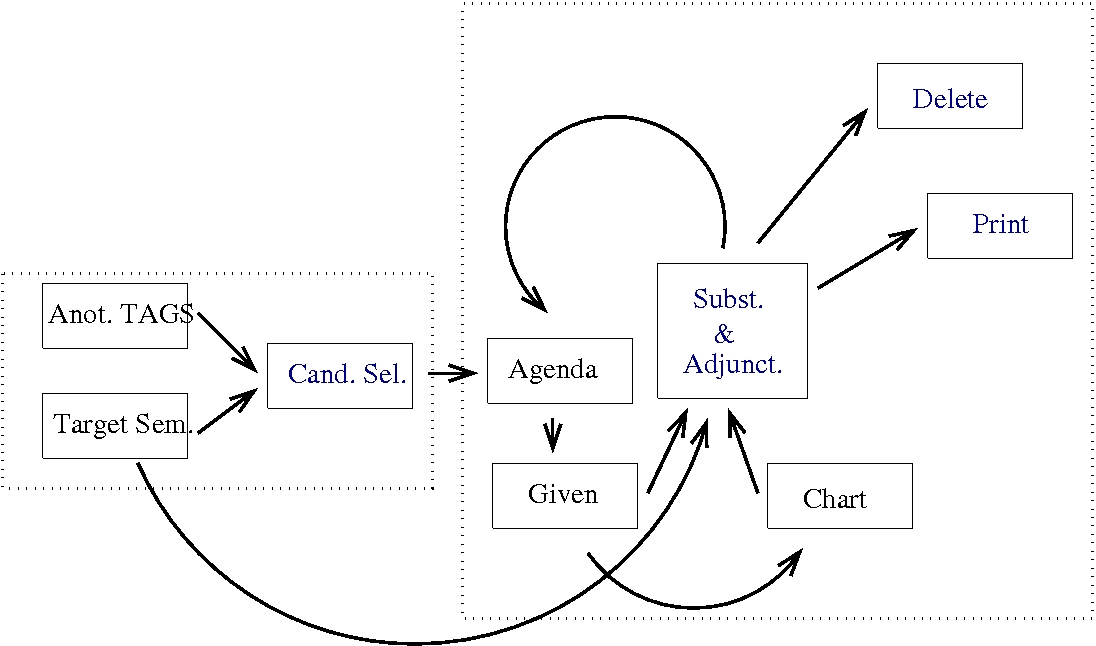
\includegraphics[scale=.32]{pics/gen.jpg}
\end{center}
\end{frame}

\end{document}
